%
% MTransformExamples.tex
%
% (c) 2019 Prof Dr Andreas Müller, Hochschule Rapperswil
%
\documentclass[tikz,11pt]{standalone}
%
% common.tex
%
% (c) 2020 Prof Dr Andreas Müller, Hochschule Rapperswil
%
\usepackage[T1]{fontenc}
\usepackage[utf8]{inputenc}
\usepackage{amsfonts}
\usepackage{amsmath}
\usepackage{amssymb}
\usepackage{times}
\usepackage{txfonts}
\usepackage{tikz}
\usetikzlibrary{arrows,intersections,math,calc,shapes.geometric,automata}
\usepackage{pgfplots}
\pgfplotsset{compat=1.16}
\usepackage{ifthen}


\begin{document}

\definecolor{blueT}{rgb}{0.6671,0.7594,0.8755}
\definecolor{CadetBlue}{cmyk}{.9,.5,0,.35}
\definecolor{gray}{cmyk}{0,0,0,.5}
\definecolor{orbits}{cmyk}{0,0,0,.7}

\def\s{1.99}
%\def\s{1.79}
\pgfmathparse{(\s/1.95)*0.32300}
\xdef\pngscale{\pgfmathresult}

\begin{tikzpicture}[>=latex, scale=\s]

\clip (-1.45,-3.55) rectangle (5.05,1.6);

\begin{scope}[]
	\def\s{1.07}
	\def\l{0.9}
	\def\ll{0.9}
	\def\lll{1.1}

	\node(ylm) at (0,0) [scale=\pngscale]{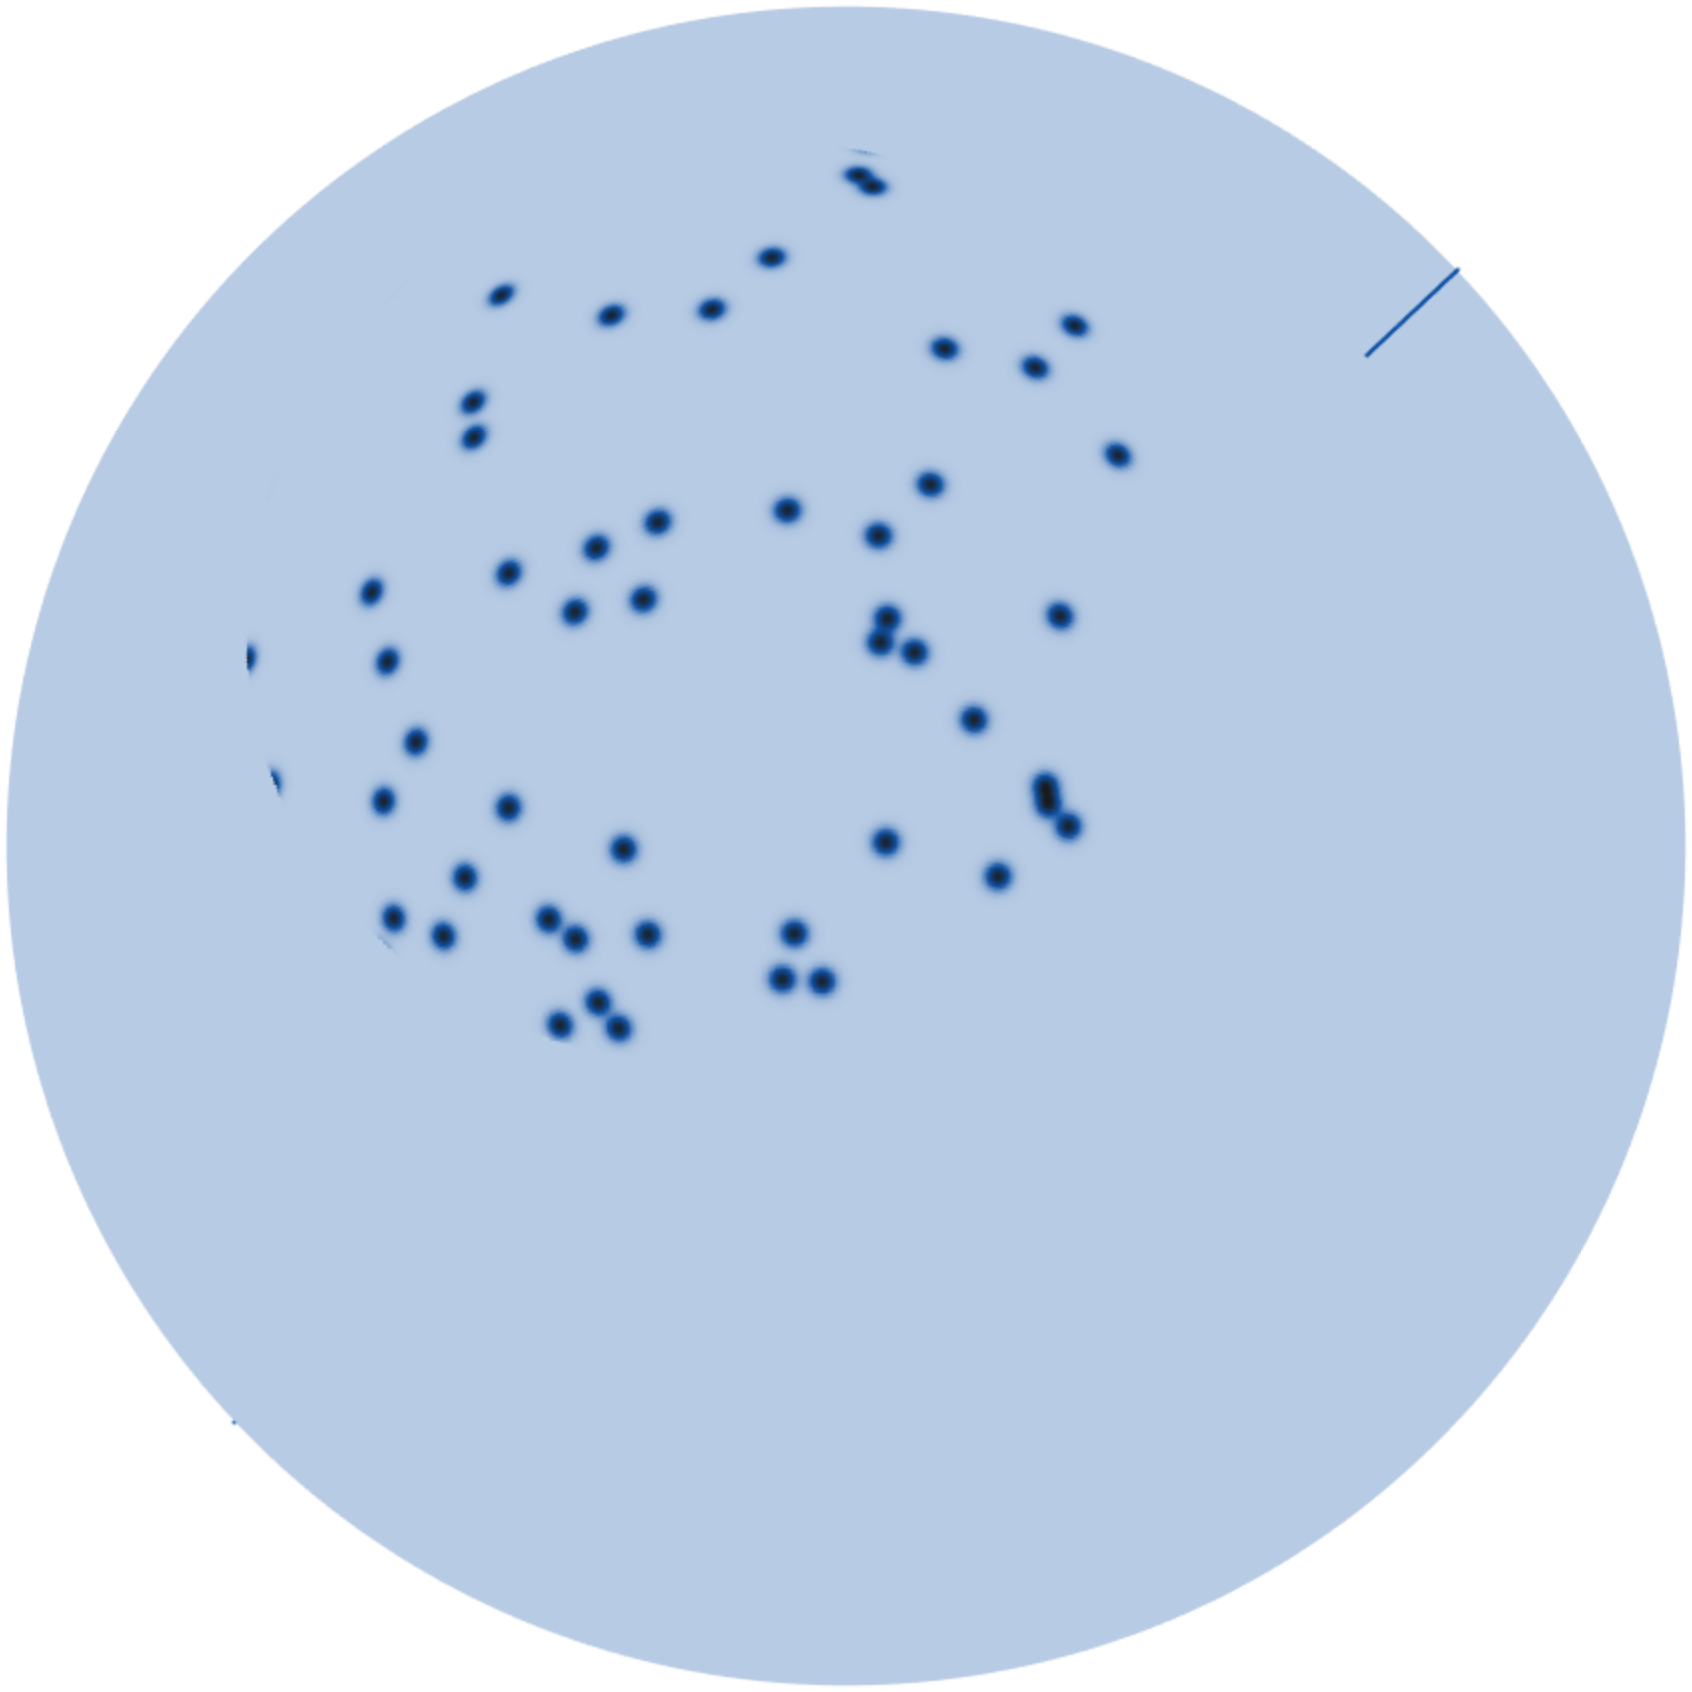
\includegraphics{f.png}};

	\def\r{1.173}
	\draw[black,fill=white,opacity=0,fill opacity=1,ultra thin]({\r*cos(32)},{\r*sin(32)})arc(32:55:\r)--++(0.2,-0.1)--cycle;
	\draw[blueT!85,fill,ultra thin]({\r*cos(32)},{\r*sin(32)})arc(32:55:\r)--++(0,-0.3)--cycle;

	% orbits
	\def\h{0.734}
	\def\ang{180}
	\def\a{0.4}
	\def\b{0.21}
	\draw[orbits,rotate=0,thin] (ylm)++(0,\h) arc(-90:-90+\ang:\a cm and \b cm);
	\draw[orbits,rotate=0,thin] (ylm)++(0,\h) arc(-90:-90-\ang:\a cm and \b cm);
	\def\h{0.373}
	\def\ang{125}
	\def\a{0.7525}
	\def\b{0.4}
	\draw[orbits,rotate=0,thin] (ylm)++(0,\h) arc(-90:-90+\ang:\a cm and \b cm);
	\draw[orbits,rotate=0,thin] (ylm)++(0,\h) arc(-90:-90-\ang:\a cm and \b cm);
	\def\h{-0.03}
	\def\ang{103}
	\def\a{	1.015}
	\def\b{0.54}
	\draw[orbits,rotate=0,thin] (ylm)++(0,\h) arc(-90:-90+\ang:\a cm and \b cm);
	\draw[orbits,rotate=0,thin] (ylm)++(0,\h) arc(-90:-90-\ang:\a cm and \b cm);
	\def\h{-0.429}
	\def\ang{93}
	\def\a{	1.155}
	\def\b{0.6}
	\draw[orbits,rotate=0,thin] (ylm)++(0,\h) arc(-90:-90+\ang:\a cm and \b cm);
	\draw[orbits,rotate=0,thin] (ylm)++(0,\h) arc(-90:-90-\ang:\a cm and \b cm);
	\def\h{-0.776}
	\def\ang{79}
	\def\a{	1.159}
	\def\b{0.61}
	\draw[orbits,rotate=0,thin] (ylm)++(0,\h) arc(-90:-90+\ang:\a cm and \b cm);
	\draw[orbits,rotate=0,thin] (ylm)++(0,\h) arc(-90:-90-\ang:\a cm and \b cm);
	\def\h{-1.03}
	\def\ang{64}
	\def\a{	1.015}
	\def\b{0.53}
	\draw[orbits,rotate=0,thin] (ylm)++(0,\h) arc(-90:-90+\ang:\a cm and \b cm);
	\draw[orbits,rotate=0,thin] (ylm)++(0,\h) arc(-90:-90-\ang:\a cm and \b cm);
	\def\h{-1.16}
	\def\ang{38}
	\def\a{0.76}
	\def\b{0.4}
	\draw[orbits,rotate=0,thin] (ylm)++(0,\h) arc(-90:-90+\ang:\a cm and \b cm);
	\draw[orbits,rotate=0,thin] (ylm)++(0,\h) arc(-90:-90-\ang:\a cm and \b cm);

	% coordinates
	\draw[gray,->, thin](ylm)++({\s*0.86*cos(-26)},{\s*0.86*sin(-26)})--++({\l*0.5*cos(-26)},{\l*0.5*sin(-26)})node[right=-2pt]{$x_2$};
	\draw[gray,->, thin](ylm)++({\s*0.86*cos(-154)},{\s*0.86*sin(-154)})--++({\l*0.5*cos(-154)},{\l*0.5*sin(-154)})node[left=-2pt]{$x_1$};
	\draw[gray,->, thin](ylm)++({\s*0.96*cos(90)},{\s*0.96*sin(90)})--++({\l*0.5*cos(90)},{\l*0.5*sin(90)})node[right=-2pt]{$x_3$};
	\draw[gray,thin](ylm)++({\s*1.096*cos(-90)},{\s*1.096*sin(-90)})--++({\ll*0.22*cos(-90)},{\ll*0.22*sin(-90)});
	\draw[gray,thin](ylm)++({\s*1.096*cos(153.5)},{\s*1.096*sin(153.5)})--++({\ll*0.22*cos(153.5)},{\ll*0.22*sin(153.5)});
	\draw[gray,thin](ylm)++({\s*1.096*cos(26.5)},{\s*1.096*sin(26.5)})--++({\ll*0.22*cos(26.5)},{\ll*0.22*sin(26.5)});

    % axis
    \draw[CadetBlue,very thick](ylm)++({\s*0.934*cos(90)},{\s*0.934*sin(90)})--++({\lll*0.5*cos(90)},{\lll*0.5*sin(90)}) node[below left=-2pt,yshift=-10]{$x$};
    \draw[CadetBlue,very thick](ylm)++({\s*(-0.934-0.163)*cos(90)},{\s*(-0.934-0.163)*sin(90)})--++({\lll*(-0.5+0.163)*cos(90)},{\lll*(-0.5+0.163)*sin(90)});
    \node at (-0.8,1.2) {$f$};

\end{scope}

\begin{scope}[xshift=3.4cm]
	\def\s{1.07}
	\def\l{0.9}
	\def\ll{0.9}
	\def\lll{1.1}

	\node(ylm) at (0,0) [scale=\pngscale]{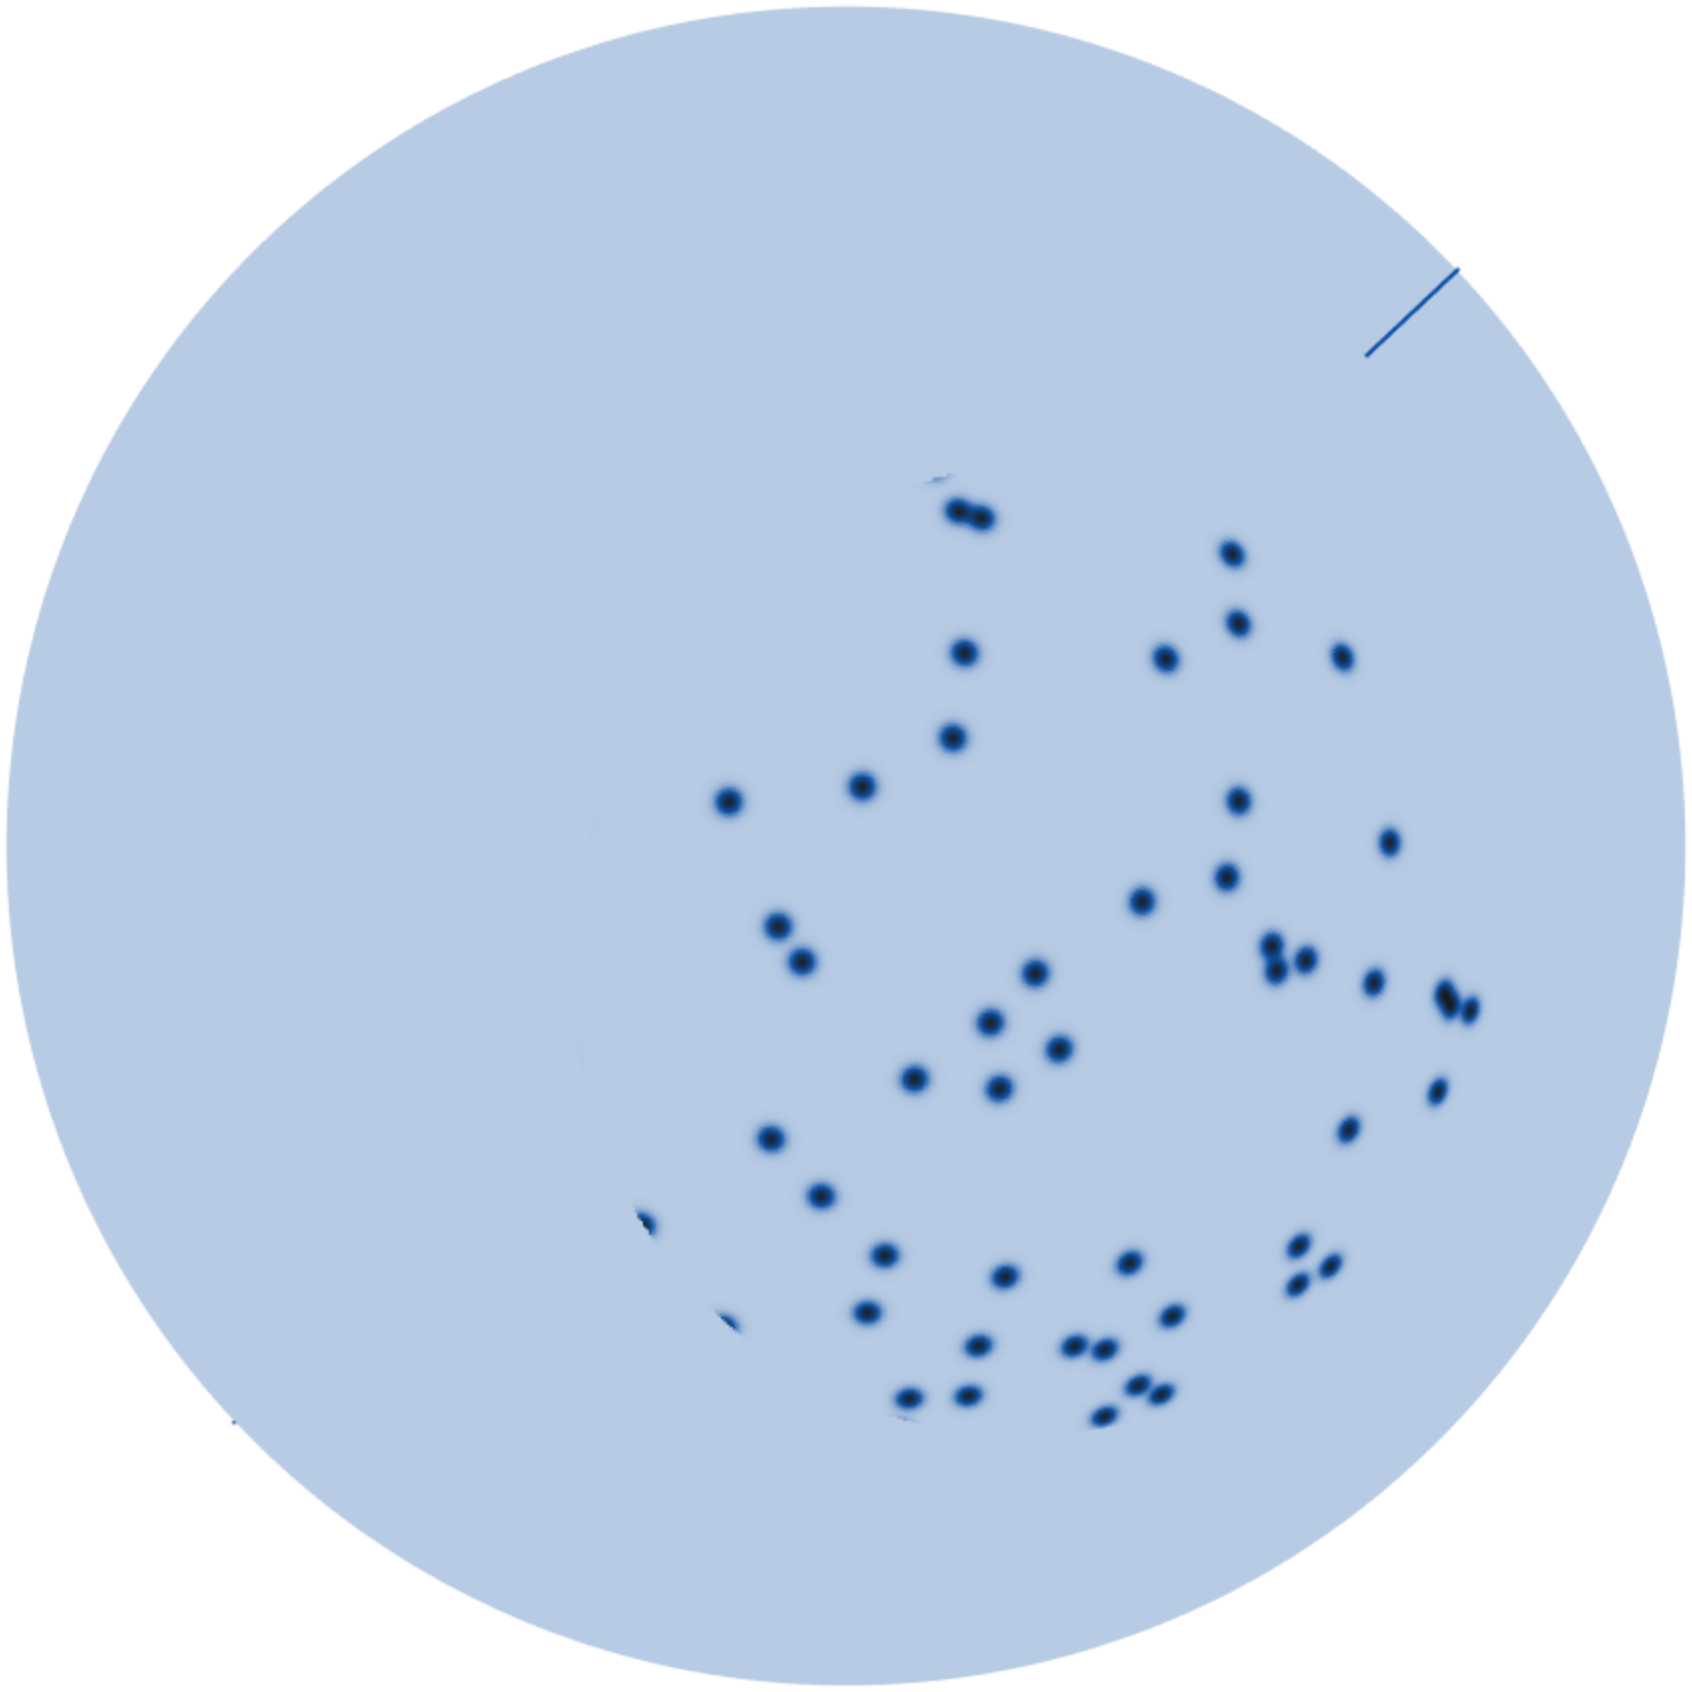
\includegraphics{g.png}};

	\def\r{1.173}
	\draw[black,fill=white,opacity=0,fill opacity=1,ultra thin]({\r*cos(32)},{\r*sin(32)})arc(32:55:\r)--++(0.2,-0.1)--cycle;
	\draw[blueT!85,fill,ultra thin]({\r*cos(32)},{\r*sin(32)})arc(32:55:\r)--++(0,-0.3)--cycle;

	% orbits
	\def\h{0.734}
	\def\ang{180}
	\def\a{0.4}
	\def\b{0.21}
	\draw[orbits,rotate=0,thin] (ylm)++(0,\h) arc(-90:-90+\ang:\a cm and \b cm);
	\draw[orbits,rotate=0,thin] (ylm)++(0,\h) arc(-90:-90-\ang:\a cm and \b cm);
	\def\h{0.373}
	\def\ang{125}
	\def\a{0.7525}
	\def\b{0.4}
	\draw[orbits,rotate=0,thin] (ylm)++(0,\h) arc(-90:-90+\ang:\a cm and \b cm);
	\draw[orbits,rotate=0,thin] (ylm)++(0,\h) arc(-90:-90-\ang:\a cm and \b cm);
	\def\h{-0.03}
	\def\ang{103}
	\def\a{	1.015}
	\def\b{0.54}
	\draw[orbits,rotate=0,thin] (ylm)++(0,\h) arc(-90:-90+\ang:\a cm and \b cm);
	\draw[orbits,rotate=0,thin] (ylm)++(0,\h) arc(-90:-90-\ang:\a cm and \b cm);
	\def\h{-0.429}
	\def\ang{93}
	\def\a{	1.155}
	\def\b{0.6}
	\draw[orbits,rotate=0,thin] (ylm)++(0,\h) arc(-90:-90+\ang:\a cm and \b cm);
	\draw[orbits,rotate=0,thin] (ylm)++(0,\h) arc(-90:-90-\ang:\a cm and \b cm);
	\def\h{-0.776}
	\def\ang{79}
	\def\a{	1.159}
	\def\b{0.61}
	\draw[orbits,rotate=0,thin] (ylm)++(0,\h) arc(-90:-90+\ang:\a cm and \b cm);
	\draw[orbits,rotate=0,thin] (ylm)++(0,\h) arc(-90:-90-\ang:\a cm and \b cm);
	\def\h{-1.03}
	\def\ang{64}
	\def\a{	1.015}
	\def\b{0.53}
	\draw[orbits,rotate=0,thin] (ylm)++(0,\h) arc(-90:-90+\ang:\a cm and \b cm);
	\draw[orbits,rotate=0,thin] (ylm)++(0,\h) arc(-90:-90-\ang:\a cm and \b cm);
	\def\h{-1.16}
	\def\ang{38}
	\def\a{0.76}
	\def\b{0.4}
	\draw[orbits,rotate=0,thin] (ylm)++(0,\h) arc(-90:-90+\ang:\a cm and \b cm);
	\draw[orbits,rotate=0,thin] (ylm)++(0,\h) arc(-90:-90-\ang:\a cm and \b cm);

	% coordinates
	\draw[gray,->, thin](ylm)++({\s*0.86*cos(-26)},{\s*0.86*sin(-26)})--++({\l*0.5*cos(-26)},{\l*0.5*sin(-26)})node[right=-2pt]{$x_2$};
	\draw[gray,->, thin](ylm)++({\s*0.86*cos(-154)},{\s*0.86*sin(-154)})--++({\l*0.5*cos(-154)},{\l*0.5*sin(-154)})node[left=-2pt]{$x_1$};
	\draw[gray,->, thin](ylm)++({\s*0.96*cos(90)},{\s*0.96*sin(90)})--++({\l*0.5*cos(90)},{\l*0.5*sin(90)})node[right=-2pt]{$x_3$};
	\draw[gray,thin](ylm)++({\s*1.096*cos(-90)},{\s*1.096*sin(-90)})--++({\ll*0.22*cos(-90)},{\ll*0.22*sin(-90)});
	\draw[gray,thin](ylm)++({\s*1.096*cos(153.5)},{\s*1.096*sin(153.5)})--++({\ll*0.22*cos(153.5)},{\ll*0.22*sin(153.5)});
	\draw[gray,thin](ylm)++({\s*1.096*cos(26.5)},{\s*1.096*sin(26.5)})--++({\ll*0.22*cos(26.5)},{\ll*0.22*sin(26.5)});

    % axis
    \draw[CadetBlue,very thick](ylm)++({\s*0.934*cos(90)},{\s*0.934*sin(90)})--++({\lll*0.5*cos(90)},{\lll*0.5*sin(90)}) node[below left=-2pt,yshift=-10]{$x$};
    \draw[CadetBlue,very thick](ylm)++({\s*(-0.934-0.163)*cos(90)},{\s*(-0.934-0.163)*sin(90)})--++({\lll*(-0.5+0.163)*cos(90)},{\lll*(-0.5+0.163)*sin(90)});
    \node at (-0.8,1.2) {$g$};

\end{scope}




\begin{scope}[]


% \draw[green](-2.5,-4)rectangle++(12.2,4);
    \begin{scope}[yshift=-3.2cm,scale=1.3]	
		\draw[->](-1.2,0)--(1.2,0)coordinate[label={$z$}];
		\draw[->](0,0)--(0,1)node[left]{$\mathcal{M}f(x)(z)$};

		\foreach \i in {-1,-0.5,...,1}{
		\draw[very thin](\i,0.05)--(\i,-0.05)node[below]{$\i$};
		}

	\draw[semithick,CadetBlue,rounded corners=0.1pt](-1,0)
	\foreach[count=\i, evaluate=\i as \x using sin(\i-90)] \y in
 {0	,
0	,
0	,
0	,
0	,
0	,
0	,
0	,
0	,
0	,
0	,
0	,
0	,
0	,
0	,
0	,
0	,
0	,
0	,
0	,
0	,
0	,
0	,
0	,
0	,
0	,
0	,
0	,
0	,
0	,
0	,
0	,
0	,
0	,
0	,
0	,
0	,
0	,
0	,
0	,
0	,
0	,
0	,
0	,
0	,
0	,
0	,
0	,
0	,
0	,
0	,
0	,
0	,
0	,
0	,
0	,
0	,
0	,
0	,
0	,
0	,
0	,
0	,
0	,
0	,
0	,
0	,
0	,
0	,
0	,
0	,
0	,
0	,
0	,
0	,
0	,
0	,
0	,
0	,
0	,
0	,
0	,
0	,
0	,
0	,
0	,
0	,
0	,
0	,
0	,
0	,
0	,
0	,
0	,
0	,
0	,
0	,
0	,
0	,
0	,
0	,
0	,
0	,
0	,
0	,
2.4693210503	,
4.1906376207	,
2.2181809943	,
1.911828488	,
2.4858402615	,
8.8589460104	,
4.6065950784	,
4.9224699311	,
6.2282364943	,
4.6160610911	,
0.9897529183	,
1.2604324849	,
5.0205187361	,
4.0922427694	,
4.8615344615	,
6.3549192666	,
3.8133222183	,
6.4744680671	,
2.6469810275	,
0.1962026078	,
0.2771028098	,
2.3705602257	,
1.8718798454	,
2.399767947	,
0.8666019528	,
2.5072820341	,
0.5367730799	,
1.05011351	,
5.7576076247	,
7.6407263019	,
7.6164526033	,
3.0273083517	,
0.277700244	,
2.1864426316	,
1.1934479395	,
0.7693308713	,
4.8246073358	,
3.3341279313	,
4.970156146	,
4.899506713	,
5.836589179	,
0.6204042774	,
0.0047297803	,
0.0001309038	,
1.36057102175659E-06	,
0.0037865197	,
0.5645165272	,
4.5468774015	,
2.1271296027	,
2.4174610234	,
6.2969672963	,
1.9996869512	,
0.5460869355	,
2.504149949	,
0.5939373162	,
0.0066926856	,
0.0001419613	,
0.0686070621	,
1.6164734888	,
1.8078016199	,
0.0959399749	,
0.0002417596	,
4.1927291278218E-07	,
1.96145069081569E-06	,
0.0018529269	,
0.306298249	,
2.4439363372	,
2.3088939423	,
2.0042842224	,
0.135581496	,
0.2130779803	,
2.32996155759437E-15	,
0	,
0	,
0	,
0}
	{
		--(\x,0.1*\y)
	};


	\end{scope}

	\begin{scope}[xshift=3.4cm,yshift=-3.2cm,scale=1.3]	

		\draw[->](-1.2,0)--(1.2,0)coordinate[label={$z$}];	
		\draw[->](0,0)--(0,1)node[left]{$\mathcal{M}g(x)(z)$};

		\foreach \i in {-1,-0.5,...,1}{
		\draw[very thin](\i,0.05)--(\i,-0.05)node[below]{$\i$};
		}

	\draw[semithick,CadetBlue,rounded corners=0.1pt](-1,0)
	\foreach[count=\i, evaluate=\i as \x using sin(\i-90)] \y in
 {0	,
0	,
0	,
0	,
0	,
0	,
0	,
0	,
0	,
0	,
0	,
0	,
0	,
0	,
0	,
0	,
0	,
0	,
0	,
0	,
0	,
0	,
0	,
0	,
0	,
0	,
0	,
0	,
0	,
0	,
0	,
0	,
0	,
0	,
0	,
0	,
0	,
0	,
0	,
0	,
0	,
0	,
0	,
0	,
0	,
0	,
0	,
0	,
0	,
0	,
0	,
0	,
0	,
0	,
0	,
0	,
0	,
0	,
0	,
0	,
0	,
0	,
0	,
0	,
0	,
0	,
0	,
0	,
0	,
0	,
0	,
0	,
0	,
0	,
0.9064294003	,
3.1129289154	,
3.1075501453	,
3.2441936143	,
5.3852535577	,
2.2825458342	,
0.7216737276	,
3.8912453094	,
6.561699276	,
8.6923533798	,
1.8300802801	,
2.27715905	,
4.8542029854	,
1.8488478094	,
4.9060787207	,
1.2599242246	,
2.0804565272	,
1.4045446341	,
1.8676110401	,
2.5230470447	,
5.1383800303	,
2.8850260458	,
0.4177632964	,
0.1451758367	,
2.6000488531	,
5.8579610558	,
3.720060494	,
2.1588742082	,
2.5645242114	,
4.8723654769	,
4.6497821453	,
2.1195203979	,
2.6091138983	,
7.2694312629	,
2.6607738772	,
2.2792976991	,
2.6346837003	,
2.2421138247	,
4.1519262997	,
3.471853332	,
7.3830857693	,
1.3854245794	,
0.0134183894	,
0.0147625459	,
0.8642695794	,
2.4081418933	,
0.3228166924	,
0.2097767363	,
2.2679984012	,
2.4886622799	,
2.2528928503	,
2.3205305954	,
2.4422139145	,
2.2123182476	,
0.2483278261	,
1.7138862083	,
4.0340555579	,
1.4283201355	,
1.7674902428	,
1.7020491385	,
0.7929707543	,
2.4746247161	,
0.4073374015	,
0.0031888091	,
0.000001274	,
1.11499472713114E-05	,
0.0089711024	,
0.7246193454	,
3.8356896968	,
2.4812565497	,
0.1534447409	,
0.3027561293	,
0	,
0	,
0	,
0	,
0	,
0	,
0	,
0	,
0	,
0	,
0	,
0	,
0	,
0	,
0	,
0	,
0	,
0	,
0	,
0	,
0	,
0	,
0	,
0	,
0	,
0	,
0	,
0	,
0	,
0	,
0	,
0	,
0	,
0	,
0}
	{
		--(\x,0.1*\y)
	};


	\end{scope}

\end{scope}

\end{tikzpicture}

\end{document}

